\begin{figure}[tbp]
\centering
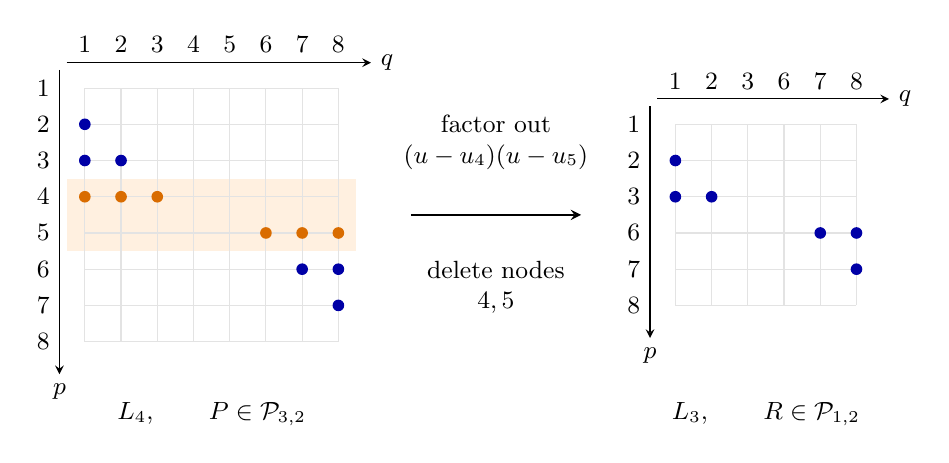
\begin{tikzpicture}[x=.46cm,y=.46cm,>=stealth,font=\small,
  kept/.style={fill=blue!65!black},
  removed/.style={fill=orange!85!black}]
  \begin{scope}
    \fill[orange!12] (.5,-5.5) rectangle (8.5,-3.5);
    \draw[step=1,gray!22] (1,-8) grid (8,-1);
    \draw[->] (.5,-.3)--(8.9,-.3) node[right] {$q$};
    \draw[->] (.3,-.5)--(.3,-8.9) node[below] {$p$};
    \foreach \i in {1,...,8} {
      \node[above] at (\i,-.3) {$\i$};
      \node[left] at (.3,-\i) {$\i$};
    }
    \foreach \p/\q in {2/1,3/1,3/2,6/7,6/8,7/8}
      \fill[kept] (\q,-\p) circle (2.1pt);
    \foreach \p/\q in {4/1,4/2,4/3,5/6,5/7,5/8}
      \fill[removed] (\q,-\p) circle (2.1pt);
    \node at (4.5,-10) {$L_4,\qquad P\in\mathcal P_{3,2}$};
  \end{scope}
  \draw[->,line width=.65pt] (10,-4.5)--(14.7,-4.5);
  \node[align=center] at (12.35,-2.5)
    {factor out\\$(u-u_4)(u-u_5)$};
  \node[align=center] at (12.35,-6.5)
    {delete nodes\\$4,5$};
  \begin{scope}[xshift=7.5cm,yshift=-.46cm]
    \draw[step=1,gray!22] (1,-6) grid (6,-1);
    \draw[->] (.5,-.3)--(6.9,-.3) node[right] {$q$};
    \draw[->] (.3,-.5)--(.3,-6.9) node[below] {$p$};
    \foreach \i/\j in {1/1,2/2,3/3,4/6,5/7,6/8} {
      \node[above] at (\i,-.3) {$\j$};
      \node[left] at (.3,-\i) {$\j$};
    }
    \foreach \p/\q in {2/1,3/1,3/2,4/5,4/6,5/6}
      \fill[kept] (\q,-\p) circle (2.1pt);
    \node at (3.5,-9) {$L_3,\qquad R\in\mathcal P_{1,2}$};
  \end{scope}
\end{tikzpicture}
\caption{The two-triangle interpolation pattern for eight nodes.
The axes record indices, not the numerical sizes of the nodes. Each
highlighted row has three points, so a polynomial
$P\in\mathcal P_{3,2}$ vanishing on $L_4$ vanishes identically on both
rows. Dividing by $(u-u_4)(u-u_5)$ gives
$R\in\mathcal P_{1,2}$, the swapped degree rectangle for six nodes.
After deleting indices $4,5$, the remaining points form $L_3$;
the right panel retains their original labels.}
\label{fig:interpolation}
\end{figure}
